\documentclass[tikz,border=12pt]{standalone}
\usepackage{amsmath,amssymb}
\usetikzlibrary{calc,arrows.meta}

\begin{document}
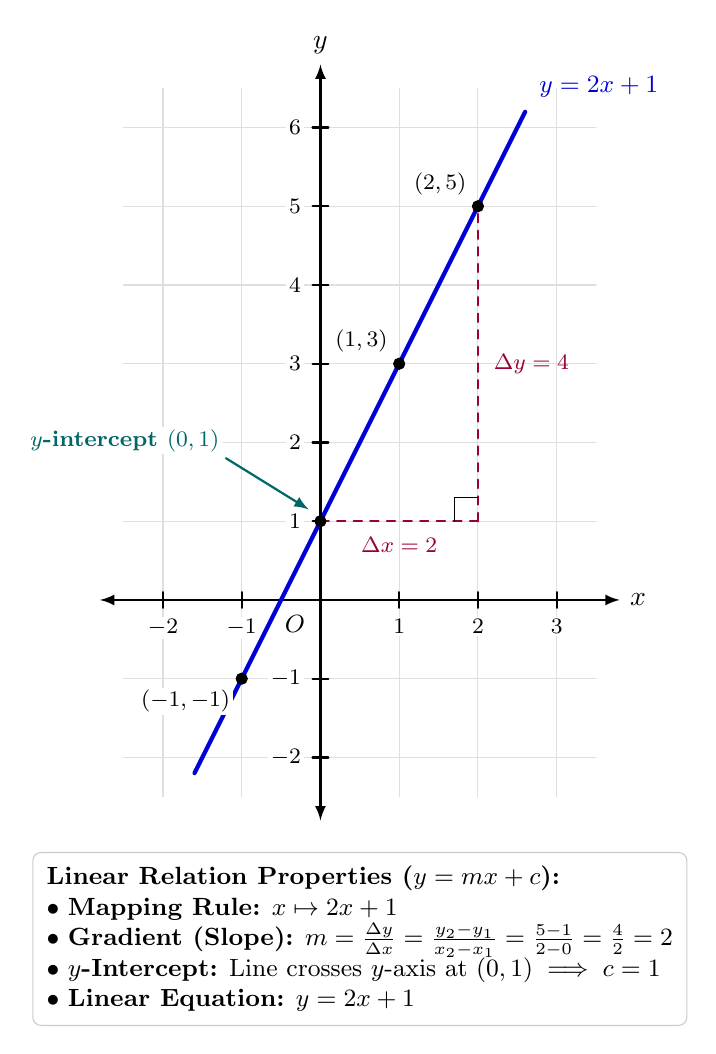
\begin{tikzpicture}[>=latex, line cap=round, line join=round]

  % Cartesian Grid
  \draw[step=1cm, gray!25, thin] (-2.5, -2.5) grid (3.5, 6.5);

  % Axes
  \draw[thick, <->] (-2.8, 0) -- (3.8, 0) node[right, font=\normalsize] {$x$};
  \draw[thick, <->] (0, -2.8) -- (0, 6.8) node[above, font=\normalsize] {$y$};

  % Origin
  \node[below left=2pt, font=\small] at (0, 0) {$O$};

  % Integer ticks on x-axis
  \foreach \x in {-2,-1,1,2,3} {
    \draw[thick] (\x, 0.1) -- (\x, -0.1);
    \node[below=3pt, font=\footnotesize, fill=white, inner sep=1pt] at (\x, -0.1) {$\x$};
  }
  % Integer ticks on y-axis
  \foreach \y in {-2,-1,1,2,3,4,5,6} {
    \draw[thick] (0.1, \y) -- (-0.1, \y);
    \node[left=3pt, font=\footnotesize, fill=white, inner sep=1pt] at (-0.1, \y) {$\y$};
  }

  % Gradient / Slope triangle between (0, 1) and (2, 5)
  \draw[thick, dashed, purple!80!black] (0, 1) -- (2, 1) node[midway, below=2pt, font=\footnotesize\bfseries] {$\Delta x = 2$};
  \draw[thick, dashed, purple!80!black] (2, 1) -- (2, 5) node[midway, right=2pt, font=\footnotesize\bfseries] {$\Delta y = 4$};
  \draw[thin] (2, 1.3) -- (1.7, 1.3) -- (1.7, 1);

  % Linear function line y = 2x + 1
  \draw[line width=1.5pt, blue!85!black] (-1.6, -2.2) -- (2.6, 6.2) node[above right=1pt, font=\small\bfseries, blue!85!black] {$y = 2x + 1$};

  % Plotted data points
  \coordinate (P1) at (-1, -1);
  \coordinate (P2) at (0, 1);
  \coordinate (P3) at (1, 3);
  \coordinate (P4) at (2, 5);

  \filldraw[black] (P1) circle (2pt) node[below left=3pt, font=\footnotesize\bfseries, fill=white, inner sep=1pt] {$(-1, -1)$};
  \filldraw[black] (P2) circle (2pt);
  \filldraw[black] (P3) circle (2pt) node[above left=3pt, font=\footnotesize\bfseries, fill=white, inner sep=1pt] {$(1, 3)$};
  \filldraw[black] (P4) circle (2pt) node[above left=3pt, font=\footnotesize\bfseries, fill=white, inner sep=1pt] {$(2, 5)$};

  % y-intercept highlight with callout tag in open Quadrant II
  \draw[thick, ->, teal!80!black] (-1.2, 1.8) node[above left=1pt, font=\footnotesize\bfseries, teal!80!black, fill=white, inner sep=1pt] {$y$-intercept $(0, 1)$} -- (-0.15, 1.15);

  % Summary Card below
  \node[align=left, font=\small, fill=white, inner sep=5pt, draw=gray!40, rounded corners=3pt, anchor=north] at (0.5, -3.2) {
    \textbf{Linear Relation Properties ($y = mx + c$):}\\
    $\bullet$ \textbf{Mapping Rule:} $x \mapsto 2x + 1$\\
    $\bullet$ \textbf{Gradient (Slope):} $m = \frac{\Delta y}{\Delta x} = \frac{y_2 - y_1}{x_2 - x_1} = \frac{5 - 1}{2 - 0} = \frac{4}{2} = 2$\\
    $\bullet$ \textbf{$y$-Intercept:} Line crosses $y$-axis at $(0, 1) \implies c = 1$\\
    $\bullet$ \textbf{Linear Equation:} $y = 2x + 1$
  };

\end{tikzpicture}
\end{document}
